% !TEX root = hw9-answers-graded.tex
\chead{\textbf{Exercises week 9}}

\begin{document}
\flushleft\textbf{Topic: Structural Causal Models}

\begin{enumerate}
  \item %(2 points) 
  Consider the structural causal model with structural equations:
  \begin{align*}
    \begin{cases}
      C & = \alpha + \beta W   \\
      N & = \gamma + \delta W,
    \end{cases}
  \end{align*}
  in which the wealth $W$ of a country is a cause of both the chocolate consumption ($C$) and the number of Nobel prizes ($N$).
  Here, $W$ is treated as an exogenous random variable with some exogenous distribution $P(W)$, while $C$ and $N$ are treated as endogenous variables. Suppose that we have a solution $(C, N, W)$ of this SCM with observational distribution $P(C, N, W)$.


  Consider the three hard interventions do$(C = c)$, do$(N = n)$, and do$(W = w)$. For each of these interventions, state which marginal distributions $P(X_i |\doit(X_j=x_j))$ for $j \in \{C, N, W\}$ and $i\in \{C, N, W\}\setminus \{j\}$ are unaffected (compare with $P(X_i)$) and which may change due to the intervention. To what extent does your answer correspond to or disagree with the intuitive causal effects between the three variables? Do you think that the provided structural equations provide a realistic model, or can they be improved?

  \begin{ungradedsolution}
    \begin{enumerate}
      \item A hard intervention do$(W = w)$ may change all variables, whereas a hard intervention on chocolate consumption or Nobel prices does not change any of the other variables:
      \begin{align*}
        P(C|\doit(W=w)) \neq P(C), & \quad P(N|\doit(W=w)) \neq P(N) \\
        P(W|\doit(C=c)) = P(W),    & \quad P(N|\doit(C=c)) = P(N)    \\
        P(C|\doit(N=n)) = P(C),    & \quad P(W|\doit(N=n)) = P(W).
      \end{align*}
      This corresponds to our intuitions on the causal effects:
      Increasing the wealth of a country may lead to more money that can be put both in chocolate and research, leading to more chocolate consumption and Nobel prices.
      However, forcing people to eat more chocolate ($\doit(C=c)$) will neither change the wealth, nor the number of Nobel prices, if our intuition is correct that chocolate does not contain brain enhancing chemicals (which aren't outweighed by the harms of too much chocolate consumption).
      For a hard intervention on Nobel prices ($\doit(N=n)$), it is less clear whether the model corresponds to our intuitions: it may be that a large number of Nobel prices increases the attractiveness of a country for researchers, thus leading to more research and thus potentially more wealth due to industry applications. So perhaps, the structural equations should have the following form:
      \begin{align*}
        \begin{cases}
          C & = \alpha + \beta W    \\
          N & = \gamma + \delta W   \\
          W & = \epsilon + \zeta N.
        \end{cases}
      \end{align*}
      In any case, we do not expect a direct effect on chocolate consumption.
    \end{enumerate}
  \end{ungradedsolution}

  \item %($8\times 1$ points)
  \begin{figure}[!b]
    \centering
    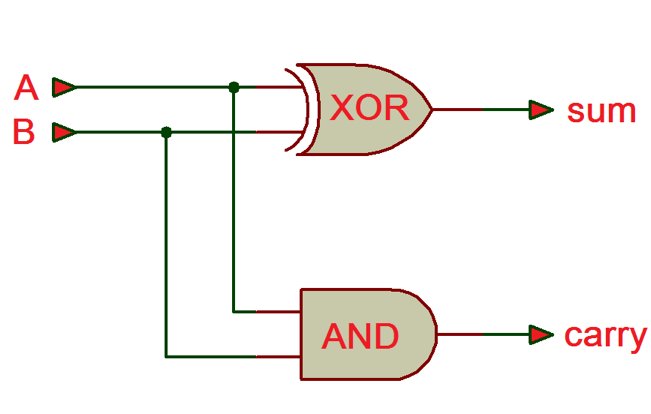
\includegraphics[width=0.6\textwidth]{half-adder-ckt}
    \caption{The half-adder is used in computers to add two bits (binary digits), with their sum represented in binary notation.
      Thus, $0 + 0 = 0$, $0 + 1 = 1$, $1 + 0 = 1$ and $1 + 1 = 10$.
      The half-adder achieves this by first computing the right-most digit, which is called the \emph{sum}, by taking the binary XOR of the two input bits.
      Additionally, the \emph{carry} is calculated since it can happen that one digit is not enough for the result, meaning we get an additional $1$ if both A and B are $1$.
      Several half-adders can be concatenated in sequence to obtain a full-adder that can sum two natural numbers that consist of multiple bits in binary notation.}
    \label{fig:half-adder}
  \end{figure}
  A so-called \emph{half-adder} is depicted in Figure \ref{fig:half-adder}. Assume that $A, B$ are binary exogenous \emph{input}-variables (in particular, they do not come equipped with a distribution).
  Use the symbol $S$ for the sum, and $C$ for the carry.

  Do the following exercises:
  \begin{enumerate}
    \item  Formally specify a structural causal model $\mathcal{M} = \left\langle J, V, W, \Xcal, P, f\right\rangle$ for the half-adder.
    \item Determine a solution function $g: \Xcal_J \times \Xcal_W \to \Xcal_V$ (see Definition \ref*{def:solution-function}). Show in this specific case that it is unique.
    \item For each combination of inputs $A$ and $B$, determine the sum and the carry.
    \item Model interventions: a hard intervention on the input A, a hard intervention on the sum S, and a soft intervention on the causal mechanism (e.g., replacing the XOR gate by an OR gate).
    What are the possible outputs of the intervened solution function $\tilde{g}$ under these interventions, and how does this differ form the possible outputs of $g$?
  \end{enumerate}

  Now, assume that $A$ and $B$ are instead binary exogenous \emph{random} variables, i.e., they are equipped with a probability distribution.
  We assume them to be independent uniformly Bernoulli distributed.

  Do the following exercises:
  \begin{enumerate}[resume*]
    \item Specify a structural causal model $\mathcal{M}'$ for this new situation.
    \item Determine the observational distribution of the random variable $(S, C)$ with values in $\{0, 1\}^2$. What is the measure-theoretic name of the operation you just performed?
    \item Perform a hard intervention on the sum $S$, forcing it to be $1$. Determine the corresponding interventional distribution of $(S, C)$.
    \item Instead, perform a hard intervention on the input $A$, forcing it to be $0$. Determine the corresponding interventional distribution of $(S, C)$.
  \end{enumerate}

  \begin{gradedsolution}
    \begin{enumerate}
      \item \points{0.5} $J=\{A, B\}, V = \{C, S\}, W = \emptyset, \Xcal_J = \{0, 1\}^{2}$, $\Xcal_V = \{0,1\}^{2}$, $\Xcal_W = \{*\}$, the set with only one point. Furthermore, $P = \delta_*$, the Dirac delta distribution, is the unique distribution on $\Xcal_W$. Finally, $f: \Xcal = \{0,1\}^{4} \to \{0,1\}^{2} = \Xcal_V$\footnote{We use, as in other exercises as well, the convention $U \times \{*\} = U$, even though, technically, this is not an equality but only an isomorphism.} is given by
      \begin{equation}
        f \begin{pmatrix} a \\ b \\ s \\ c \end{pmatrix} = \begin{pmatrix} a \oplus b \\ a \wedge b\end{pmatrix}.
        \label{eq:causal_mechanism_half_adder}
      \end{equation}
      \item \points{0.5} Assume we had a solution $g: \Xcal_J\times \Xcal_W = \{0,1\}^2 \to \{0,1\}^2 = \Xcal_V$.
      By definition of a solution function, this would mean that we have for all $a, b \in \{0,1\}$ the following string of equalities:
      \begin{equation}
        \begin{pmatrix} g_S \begin{pmatrix} a \\ b\end{pmatrix} \\ g_C \begin{pmatrix} a \\ b \end{pmatrix}\end{pmatrix}
        = g \begin{pmatrix} a \\ b\end{pmatrix}
        = f \begin{pmatrix} a \\ b \\ g \begin{pmatrix} a \\ b\end{pmatrix}\end{pmatrix}
        = \begin{pmatrix} a \oplus b \\ a \wedge b\end{pmatrix},
        \label{eq:string_of_equations}
      \end{equation}
      which forces the equalities $g_S \begin{pmatrix} a \\ b\end{pmatrix} = a \oplus b$ and $g_C \begin{pmatrix} a \\ b\end{pmatrix} = a \wedge b$.
      This shows uniqueness, and by construction, this is indeed a valid solution function.
      \item \points{0.5} We can just plug in all combinations of input bits into our solution function in order to determine the sum and the carry. Remember that the sum is given by the upper entry, and the carry by the lower entry, of the results:
      \begin{equation}
        g \begin{pmatrix} 0 \\ 0\end{pmatrix} = \begin{pmatrix} 0 \\ 0\end{pmatrix}, \quad
        g  \begin{pmatrix} 1 \\ 0\end{pmatrix} = \begin{pmatrix} 1 \\ 0\end{pmatrix}, \quad
        g  \begin{pmatrix} 0 \\ 1\end{pmatrix} = \begin{pmatrix} 1 \\ 0\end{pmatrix}, \quad
        g \begin{pmatrix} 1 \\ 1\end{pmatrix} = \begin{pmatrix} 0 \\ 1\end{pmatrix}
        \label{eq:sums_and_carries}
      \end{equation}
      \item \points{0.5} Hard intervention on the input $A$: if we set $A = 0$, then this leaves us only with the two possibilities above in which the first input of $g$ is $0$, and similarly for $A = 1$.
      In the same way, if we do a hard intervention on $B$, then we cut away half of the possibilities.
      Note that forcing either $A$ or $B$ to be zero automatically means that the carry is zero as well.
      For the soft intervention on the causal mechanism, replacing the XOR gate with an OR gate, we obtain the following solution function:
      \begin{equation}
        \tilde{g} \begin{pmatrix} a \\ b\end{pmatrix} = \begin{pmatrix} a \lor b \\ a \land b \end{pmatrix}.
        \label{eq:new_solution_function}
      \end{equation}
      In this case, the following are the results of applying the solution function to all input bit combinations:
      \begin{equation}
        \tilde{g} \begin{pmatrix} 0 \\ 0\end{pmatrix} = \begin{pmatrix} 0 \\ 0\end{pmatrix}, \quad
        \tilde{g}  \begin{pmatrix} 1 \\ 0\end{pmatrix} = \begin{pmatrix} 1 \\ 0\end{pmatrix}, \quad
        \tilde{g} \begin{pmatrix} 0 \\ 1\end{pmatrix} = \begin{pmatrix} 1 \\ 0\end{pmatrix}, \quad
        \tilde{g} \begin{pmatrix} 1 \\ 1\end{pmatrix} = \begin{pmatrix} 1 \\ 1\end{pmatrix},
        \label{eq:adapted_concrete_solutions}
      \end{equation}
      which, as you can see, only changes the very last result.
      \item \points{0.5} $J' = \emptyset, V' = \{S, C\}, W' = \{A, B\}, \Xcal_{J'}' = \{*\}$, $\Xcal_{V'}' = \{0,1\}^{2}$, $\Xcal_{W'}' = \{0,1\}^{2}$, $P': \Bcal_{W'} \to [0,1], U \mapsto \frac{\# U}{4}$, and $f': \{0,1\}^{4} \to \{0,1\}^{2}$ is given by
      \begin{equation}
        f' \begin{pmatrix} s \\ c \\ a \\ b \end{pmatrix} = \begin{pmatrix} a \oplus b \\ a \land b \end{pmatrix}.
        \label{eq:probabilistic_case}
      \end{equation}
      \item \points{0.5} Let $P_{(S,C)}$ the observational distribution of the random variable $(S,C)$. Let $p_{(S,C)}$ its probability mass function.
      Then, as can easily be checked, we obtain $p_{(S,C)}\begin{pmatrix} 0 \\ 0 \end{pmatrix} = \frac{1}{4}$, $p_{(S,C)}\begin{pmatrix} 1 \\ 0 \end{pmatrix} = \frac{1}{2}$, $p_{(S,C)}\begin{pmatrix} 0 \\ 1 \end{pmatrix} = \frac{1}{4}$, $p_{(S,C)}\begin{pmatrix} 1 \\ 1 \end{pmatrix} = 0$.
      This mass function then fully determines the probability measure $P_{(S,C)}$.
      Formally, if $g': \Xcal'_{W'} = \{0,1\}^{2} \to \{0,1\}^{2} = \Xcal'_{V'}$ is a solution function of the SCM $\mathcal{M}'$, then $P_{(S,C)} = (g')_*P'$ is the push-forward measure of the exogenous distribution $P'$.
      \item \points{0.5} $P_{(S,C)}\left( \begin{pmatrix} 1 \\ 0 \end{pmatrix} \middle| \text{do}(S=1)\right) = \frac{3}{4}$, $P_{(S,C)}\left( \begin{pmatrix} 1 \\ 1 \end{pmatrix} \middle| \text{do}(S=1)\right) = \frac{1}{4}$
      \item \points{0.5} $P_{(S,C)}\left( \begin{pmatrix} 0 \\ 0 \end{pmatrix} \middle| \text{do}(A=0)\right) = \frac{1}{2}$,   $P_{(S,C)}\left( \begin{pmatrix} 1 \\ 0 \end{pmatrix} \middle| \text{do}(A=0)\right) = \frac{1}{2}$
    \end{enumerate}
  \end{gradedsolution}

\end{enumerate}

\end{document}
